\chapter{Introduction}

\section{Problem Definition}
\pagestyle{headings}

Before moving to what has been done in this thesis I wish to briefly discuss the setup of our channel flow and the equations used to solve the problem.

\begin{figure}[h]
\centering
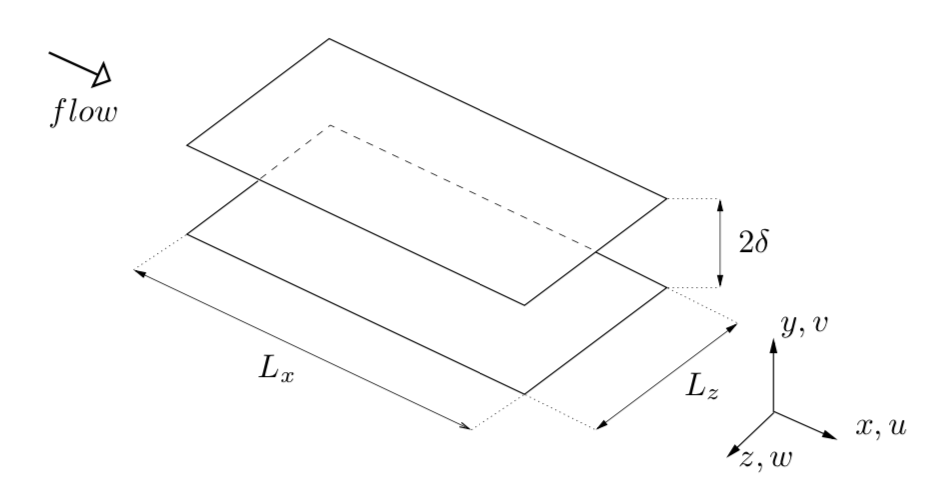
\includegraphics[width=0.8\textwidth]{grafici/sketch_dominio}
\caption{Domain of interest}
\label{sketch_dominio}
\end{figure}

We have the domain sketched in figure~\ref{sketch_dominio} where the $x$ and $z$ coordinates denote the streamwise and spanwise directions of the flow, while the $y$ coordinate is the wall normal ones.
Along these three dimension we have $u,v$ and $w$ components of velocity.

The flow is assumed to be periodic in the streamwise and spanwise directions. The lower wall is at position $y_l$ and the upper wall at position $y_u$. The reference length $\delta$ is taken to be one half of the channel height.
Once an appropriate reference velocity is chosen, we can define the Reynolds number as:
\[
Re = \frac{U\delta}{\nu}
\]
where $\nu$ is the kinematic viscosity of the fluid.

According to our geometry and the assumption of incompressible flow, we can express the behavior of the flow through the mass conservation law and the Navier-Stokes equations, which in a dimensionless form states:\\
\begin{equation}
\frac{\partial u}{\partial x} + \frac{\partial v}{\partial y} + \frac{\partial w}{\partial z}
\label{mass:cons}
\end{equation}
\begin{subequations}
\label{eqn:ns}
\begin{align}
\frac{\partial u}{\partial t} + u\frac{\partial u}{\partial x} + v\frac{\partial u}{\partial y} + w\frac{\partial u}{\partial z} &= 
- \frac{\partial p}{\partial x} + \frac{1}{Re} \nabla^{2}u  \\
\frac{\partial v}{\partial t} + u\frac{\partial v}{\partial x} + v\frac{\partial v}{\partial y} + w\frac{\partial v}{\partial z} &= 
- \frac{\partial p}{\partial y} + \frac{1}{Re}\nabla^{2}v\\
\frac{\partial w}{\partial t} + u\frac{\partial w}{\partial x} + v\frac{\partial w}{\partial y} + w\frac{\partial w}{\partial z} &= 
- \frac{\partial p}{\partial z} + \frac{1}{Re}\nabla^{2}w
\end{align}
\end{subequations}
The differential problem is closed when an initial condition for all the fluid variables is specified, and suitable boundary conditions are chosen. At the wall the no-slip condition is imposed.





\section{Wall normal vorticity and velocity~equations}
The numerical method does not rely on the equations~\eqref{eqn:ns}, instead it solve the wall-normal velocity and the wall-normal vorticity equations, recovering, at the end of the the solution, the three velocity components.
Defining the wall-normal component of the vorticity vector as:
\[
\eta = \frac{\partial u}{\partial z} - \frac{\partial w}{\partial x}
\]
which, in Fourier space, holds:
\[
\hat{\eta} = i\beta \hat{u} - i \alpha \hat{w}
\] 
with the hat indicating Fourier-transformed quantities, $i$ the imaginary part, $\alpha$ and $\beta$ the streamwise and spanwise wave numbers; it is possibile to write a one-dimensional second-order evolutive equation for $\hat{\eta}$ which does not involve pressure, as proposed in \cite{kim_moin_moser}.

Taking the y component of the curl of the momentum equation we obtain:
\begin{equation}
\frac{\partial \hat{\eta}}{\partial t}  = \frac{1}{Re}  \big( D_{2}(\hat{\eta}) - k^{2} \hat{\eta} \big) + i \beta \widehat{HU} -i \alpha \widehat{HW}
\end{equation}
where $D_{2}$ is the second derivative in the wall-normal direction, $k^{2}$ is the sum of $\alpha$ and $\beta$, and the nonlinear terms are defined as:
\begin{subequations}
\widehat{HU} = i \alpha \widehat{uu} + D_{1} \widehat{uv} + i \beta \widehat{uw}

\end{subequations}


 that can be used in substitution of the \eqref{eqn:ns}

Further informations are available in \cite{cpl:presentazione}






\section{Numerical Method}
the engine of Quadrio and Luchini described into~\cite{cpl:presentazione} which works per \emph{y-slabs}, as shown in figure~\ref{domain_decomp},
\begin{figure}
\centering
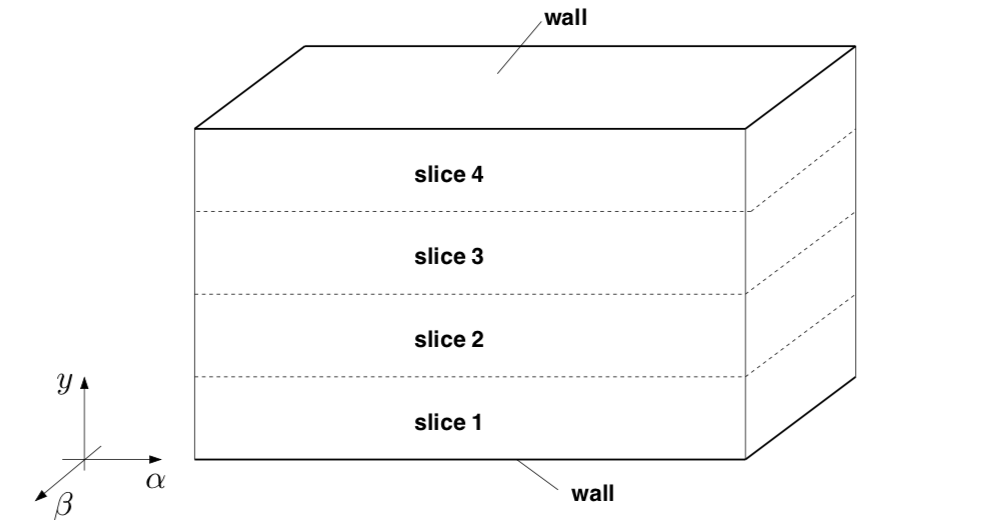
\includegraphics[width=0.5\textwidth]{grafici/decomp_dominio_cpl}
\caption{Original domain decomposition in case of 4 processors}
\label{domain_decomp}
\end{figure} allowing to perform the convolutions and relatives Fourier transformations locally on each processor, leading to a minimum of communication, moving to communication intensive decompositions, such as \emph{z-slabs}, \emph{x-slabs} or \emph{pencils}.

These solutions require communication to perform the array transpose needed by the FFTs in the two homogeneous directions